\section{Обзор предметной области}
\label{sec:domain:intro}

В данном разделе будет произведён обзор программых средств аналогичных разрабатываемому в рамках дипломного проекта - определение психологических параметров человека по образцу почерка, а так же литературных источников. Проанализированны преимущества и недостатки различных подходов к выделению и классификации признаков рукописного текста.

\subsection{Графология}
\label{sub:domain:grafologic}
\emph{Графология} - это учение, постулирующее наличие устойчивой связи месту почерком и индивидуальными особенностями личности.

Идея использования почерка для выявления психологических параметров личности впервые была предложена в 1622 в книге итальянского профессора Камилло Бальдо <<Как узнать природу и качества человека, взглянув на букву, которую он написал>> ~\cite{kamillo_grafology}. Первым кто систематизировал знания стал Фландрэна аббат Мишон в 1872 году. Он проанализировал большое количество работ по графологии и образцов почерка и в своей книге <<Систeмa графологии>> предложил \emph{метод Мишона}, он основывался на анализе штрихов, букв, слов, свободных движений, строк и пр.~\cite{mishon_grafology}

Начиная с середины 20 века графология начала рассматриваться как псевдонаучное учение~\cite{graphology_wiki}. По результатам исследования профессионалльным графологам не удалось достоверно оценить трудовые способности человека. В среднем профессиональные графологи давали такую же по степени достоверности оценку, как и люди «с улицы»~\cite{neter_shakhar_psevdograph}~\cite{king_koehler_psevdograph}. В десятках исследований было показано отсутствие связи особенностей почерка с трудовыми способностями человека.

Тем не менее графология широко используется в современной практике отбора кадров~\cite{graphology_psyfactor}.

Основные признаки почерка, которые анализирует графологическая экспертиза:
\begin{enumerate}
  \item размер букв (очень маленькие, маленькие, средние, крупные);
  \item наклон букв (левый наклон, легкий наклон влево, правый наклон, резкий наклон вправо);
  \item направление почерка: (строчки ползут вверх, строчки прямые,  строчки ползут вниз);
  \item размашистость и сила нажима: (легкая, средняя, сильная, очень сильная);
  \item характер написания слов (склонность к соединению букв и слов, склонность к отдалению букв друг от друга, смешанный стиль);
  \item общая оценка (почерк старательный, почерк неровный, почерк небрежный, почерк неразборчивый).
\end{enumerate}

Перечисленные параметры почерка являются устойчивыми, но все же присутсвует естественные отклонения параметров (длина, ширина, толщина, угол) от средних значений. Вариация становится наиболее заметной при изменение психоогического состояния человека, например при страхе, беспокойстве, алкогольном опъянении.

\subsection{Анализ аналогов}
\label{sub:domain:analogs}

\subsubsection{ScriptAlyzeR}
\label{sub:domain:analogs:neuro_script} 

Программое средство <<ScriptAlyzeR>> является частью семейства программых средств для работы с рукописным текстов компании <<NeuroScript>> и представляет собой декстопное приложение для операционных систем Windows~\cite{analogs_scriptAlyzer}.

Основными возможностями ПС являются:
\begin{itemize}
	\item Мультимодальные движения. Положение ручки, давление, ориентация, положение мыши и положение пальца на 100-200 Гц;
	\item Бимануальные движения. Измеряйте координацию, записывая одновременно две ручки;
	\item Real-Time, Real-Size Обратная связь. Для планшетных компьютеров и планшетов. Отображение и печать в реальном размере;
	\item Изменение толщины линии. Непосредственная визуальная и звуковая обратная связь с пером;
	\item Искаженная визуальная обратная связь. Поворот, перекос и отражение на мониторе компьютера в режиме реального времени;
	\item Моделирование. Генерировать рукописные цифровые данные с шумом с известными характеристиками штрихов для проверки точности обработки;
	\item Проверка непротиворечивости. Проверяйте каждое испытание, когда оно записано;
	\item Знание результатов. Покажите участникам, насколько хорошо они после каждого испытания показали максимальную производительность и стабильность;
	\item Многостраничные записи. Разделить текст на слова и штрихи;
	\item Внешние приложения. Полная интеграция с вашими собственными модулями с использованием сценариев MATLAB® или скомпилированных программ;
	\item Оптически сканированные изображения. Сегмент в визуальные штрихи и оценка характеристик за такт;
	\item Изображение для движения. Сканируйте Архимеды спиралями из бумаги и проанализируйте их как последовательность движения.
\end{itemize}

Основными недостатками ПС являются:
\begin{itemize}
  \item Поддерка только ОС семейства Windows (XP, 7, 8)
  \item Платное использование (799+ US\$)
\end{itemize}

Согласно утверждениям разработчиков ПС может быть использовано для оценки моторных функций, диагностики нейрологических отклонений, а так же тестирования на состояние алкогольного опъянения.

\begin{figure}[ht]
    \centering
    \label{fig:domain:analogs:neuro_script}
    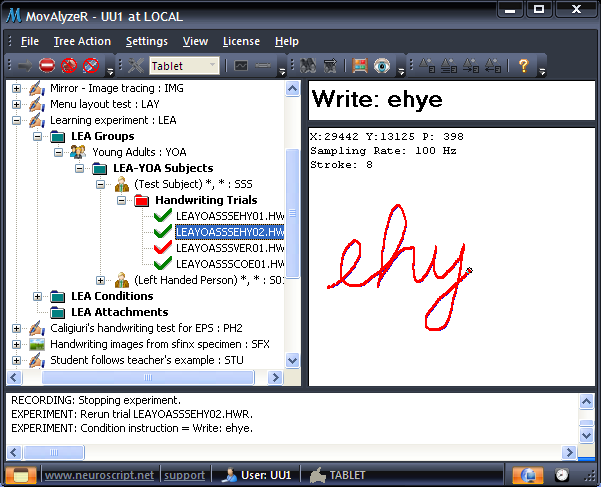
\includegraphics[width=0.7\textwidth]{figures/neuroscript.png}
    \caption{Программое средство <<ScriptAlyzeR>>}
\end{figure}

\subsubsection{Graphology}
\label{sub:domain:analogs:graphology} 

Программое средство <<Graphology>> является приложение для операционной системы Android разработанным компанией <<LH Apps>>~\cite{analogs_graphology}.

Программное средство <<Graphology>> предназначена для анализа почерка и определения характеристик личности. Алгоритм работы программы основан на обширных исследованиях и был создан при консультации профессиональных экспертов графологии.

Основными возможностями ПС являются:
\begin{itemize}

  \item Поддержка ОС Android;
  \item Многофакторная оценка параметров личности (почерк, подпись, рисунки);
  \item Выполнение анализа без доступа в интернет.
\end{itemize}

Основными недостатками ПС являются:
\begin{itemize}
  \item Поддержка только ОС Android;
  \item Поддержка только английского языка;
  \item Для ввода образцов почерка используется экран смартфона, что приводит к искажению в написании символов при низком разрешении и без использование стилуса.
\end{itemize}

\begin{figure}[ht]
    \centering
    \label{fig:domain:analogs:graphology}
    
\includegraphics[width=0.7\textwidth]{figures/graphology_analog.jpeg}
    \caption{Программое средство <<Graphology>>}
\end{figure}

\subsubsection{Signature Analysis}
\label{sub:domain:analogs:signature_analysis} 

Программое средство <<Signature Analysis>> является приложение для операционной системы Android разработанным компанией <<Beyond Consultancy Services>>~\cite{analogs_signature_analysis}.

Программное средство <<Signature Analysis>> предназначена определения характеристик личности по образцу подписи. В разработке учавствовал графолог с многолетним опытом, выступающей в качестве консультанта многих крупных компаний.

Основными возможностями ПС являются:
\begin{itemize}
  \item Поддержка ОС Android;
  \item Широкий спектр анализируемых параметров подписи (скорость, давление, длины, направления);
\end{itemize}

Основными недостатками ПС являются:
\begin{itemize}
  \item Поддержка только ОС Android;
  \item Платный анализ каждой подписи (0,83 US\$);
  \item Для работы необходимо инернет соединение;
  \item Для ввода образцов почерка используется экран смартфона, что приводит к искажению в написании символов при низком разрешении и без использование стилуса.
\end{itemize}

\begin{figure}[ht]{}
    \centering
    \label{fig:domain:analogs:signature_analysis}
    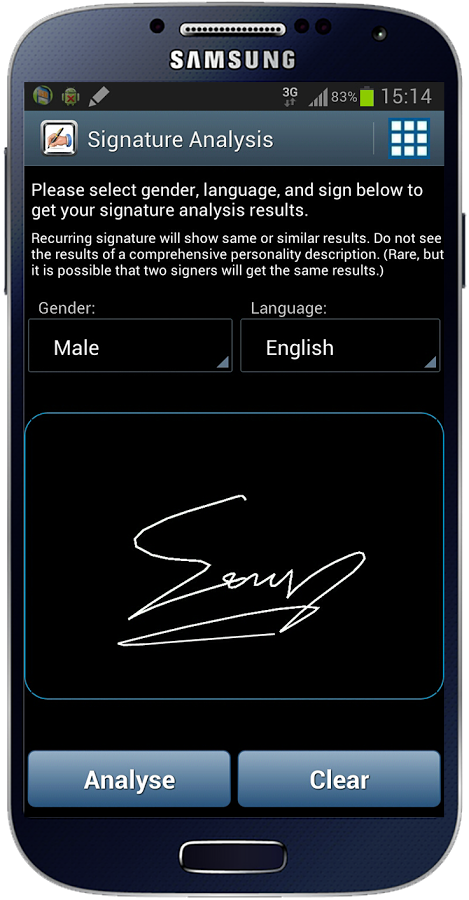
\includegraphics[height=0.5\textheight]{figures/analog_signature_analysis.png}
    \caption{Программое средство <<Signature Analysis>>}
\end{figure}

\subsubsection{My Graphology}
\label{sub:domain:analogs:my_graphology}

Программое средство <<My Graphology>> является приложение для операционной системы Android разработанным компанией <<PENS>>~\cite{analogs_my_graphology}.

Основными возможностями ПС являются:
\begin{itemize}
  \item Поддержка ОС Android;
  \item Использовать для ввода экран или фотографию почерка;
  \item Выполнение анализа без доступа в интернет.
\end{itemize}

Основными недостатками ПС являются:
\begin{itemize}
  \item Поддержка только ОС Android;
  \item В разработке не учавствовали эксперты графологи;
  \item Поддержка только испанского языка интерфейса.
\end{itemize}

\begin{figure}[ht]
    \centering
    \label{fig:domain:analogs:my_graphology}
    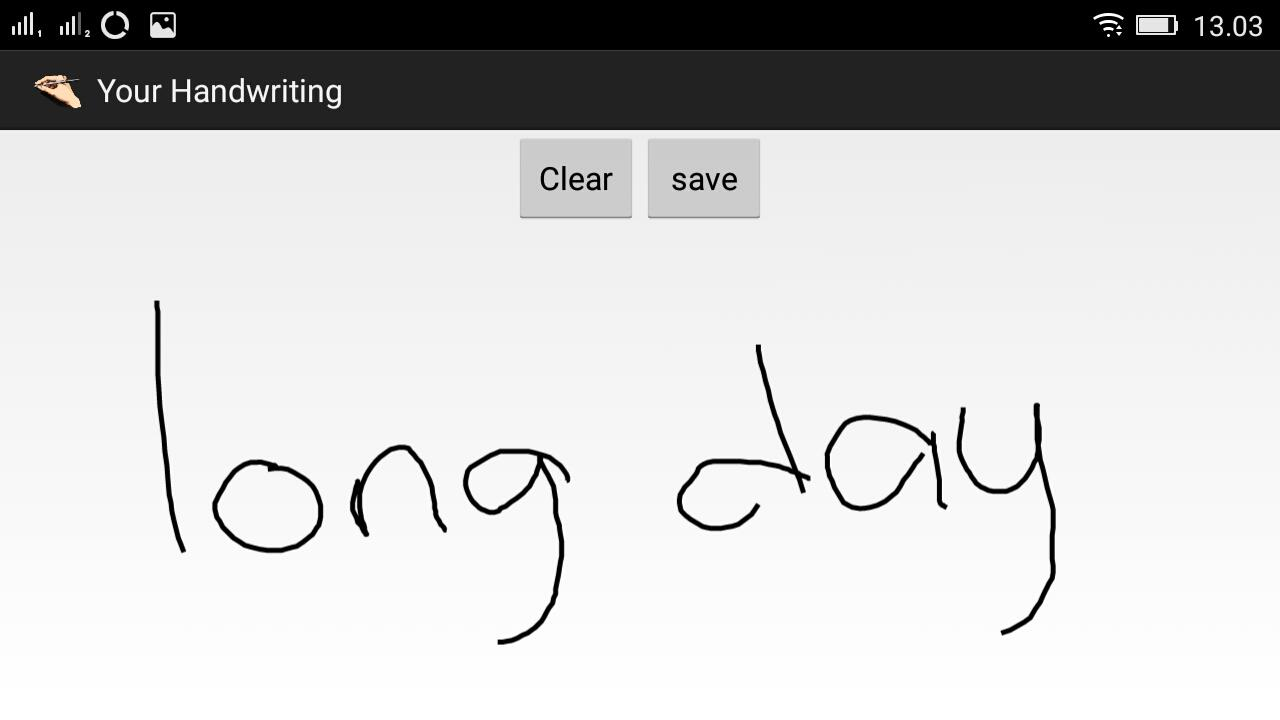
\includegraphics[width=0.55\textwidth]{figures/analog_my_graphology.jpeg}
    \caption{Программое средство <<My Graphology>>}
\end{figure}

\subsubsection{GRAPHOLOGY signature analysis}
\label{sub:domain:analogs:graphology_sign_analysis}

Программое средство <<GRAPHOLOGY signature analysis>> является приложение для операционной системы Android разработанным компанией <<DokThor>>~\cite{analogs_graphology_sign_analysis}. Программное средство <<GRAPHOLOGY signature analysis>> предназначена определения характеристик личности по образцу подписи.

Основными возможностями ПС являются:
\begin{itemize}
  \item Поддержка ОС Android;
  \item Выполнение анализа без доступа в интернет;
  \item Предоставление характеристик по личности по 5 основным критериям.
\end{itemize}

Основными недостатками ПС являются:
\begin{itemize}
  \item Поддержка только ОС Android;
  \item В разработке не учавствовали эксперты графологи;
  \item Механизм ввода подписи неочевиден;
  \item Для ввода образцов почерка используется экран смартфона, что приводит к искажению в написании символов при низком разрешении и без использование стилуса.
\end{itemize}

\begin{figure}[ht]
    \centering
    \label{fig:domain:analog:graphology_sign_analysis}
    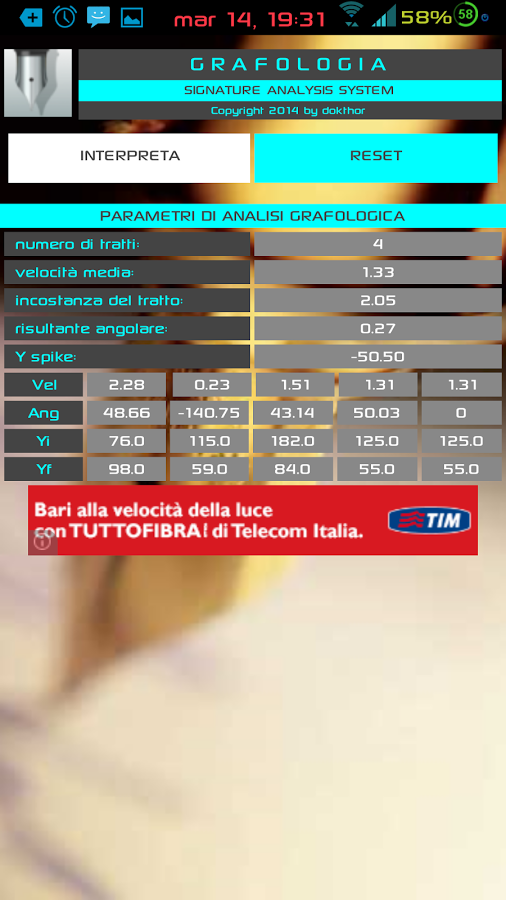
\includegraphics[height=0.5\textheight]{figures/analog_graphology_sign_analysis.png}
    \caption{<<GRAPHOLOGY signature analysis>>}
\end{figure}

\subsubsection{Graphology Lite}
\label{sub:domain:analogs:graphology_lite}

Программое средство <<Graphology Lite>> является приложение для операционной системы Android разработанным компанией <<Hyperborea>>~\cite{analogs_graphology_sign_analysis}.

Основными возможностями ПС являются:
\begin{itemize}
  \item Поддержка ОС Android;
  \item Выполнение анализа без доступа в интернет;
  \item Использовать для ввода экран или фотографию почерка.
\end{itemize}

Основными недостатками ПС являются:
\begin{itemize}
  \item Поддержка только ОС Android;
  \item В разработке не учавствовали эксперты графологи;
  \item Бесплатная версия позволяет произвести анализ только одного образца. Платная версия стоит 1.05 US\$.
\end{itemize}

\begin{figure}[ht]
    \centering
    \label{fig:domain:analogs:graphology_lite}
    
\includegraphics[height=0.5\textheight]{figures/analog_graphology_lite.png}
    \caption{Программое средство <<Graphology Lite>>}
\end{figure}

\subsection{Анализ литературных источников}
\label{sub:domain:literary_sources}

\subsection{Использование PUF для идентификации и аутентификации цифровых устройств}
\label{sub:domain:puf_auth}
Аутентификация традиционно характеризуется как процесс проверки того, что сущность владеет конкретной информацией, например, паролем, обладает конкретными свойствами, или же является именно тем, за что себя выдает. Многофакторная аутентификация представляет собой комбинацию этих проверок. Аутентификация на основе физически неклонируемых функций подразумевает наличие разных независимых устройств, каждое из которых характеризуется набором паролей (т.е. в данном случае -- набором пар запрос"=ответ), который однозначно идентифицирует эти устройства, то есть, в какой-то степени, аутентификацию на основе PUF можно считать многофакторным механизмом.

Множество возможных применений ФНФ также включает шифрование информации, обнаружение вредоносных изменений структуры интегральной микросхемы, контроль специфических функций устройств и многие другие. Каждый из сценариев использования предъявляет определенные требования к свойствам используемой ФНФ. В частности, для использования в криптографических целях, ФНФ должна быть устойчива к атакам моделирования, т.е. должна препятствовать построению более-менее точной модели своей структуры и/или поведения. Это же применимо и к протоколам аутентификации на основе ФНФ. Общее правило -- чем больше контроля над своими входными и выходными параметрами ФНФ предоставляет приложению, тем лучше оно должно быть защищено от таких атак.

Применительно к аутентификации на основе ФНФ применяют термины \emph{электронный ключ (токен)} -- для обозначения утройства, оснащённого ФНФ, чья подлинность проверяется, например, смарт-карта или RFID-метка~\cite{rfid_puf}, и \emph{доверенный сервер} -- для обозначения стороны, располагающей истинными данными идентификации конкретных устройств.

Существует два основных подхода к осуществлению системы аутентификации, основанной на физически неклонируемых функциях. Первый подход состоит в получении стойкого и безопасного криптографического ключа из ответа физически неклонируемой функции и использовании этого ключа в каком"=либо из протоколов аутентификации. В этом случае ФНФ используется в качестве или как составная часть генератора истинно случайных чисел с показателями, достаточными для его применения в криптографических целях. Секретность ключа повышается тем, что в открытом виде могут храниться только данные, использованые для его генерации, в данном случае -- наборы пар. Следовательно, воспроизвести ключ возможно только при использовании исходной ФНФ и с данным набором входных данных. Для этого подхода достаточно довольно простой ФНФ (т.н. \emph{weak PUF, слабая ФНФ}), способной сгенерировать достаточное для построения ключа количество случайной информации, но при этом устройство должно содержать реализацию криптографического алгоритма, чтобы из входного набора сконструировать ключ. К сожалению, этот метод уязвим к атаке по стороннему каналу (\emph{side-channel attack}): злоумышленник может получить секретный ключ, используя уязвимости в аппаратной реализации алгоритма~\cite{pufbased_auth,puf_cryptography}.

Другой подход состоит в разработке схемы аутентификации, которая напрямую применяет уникальность и непредсказуемость поведения пары запроса"=ответа отдельного объекта. Такая схема состоит из двух фаз (регистрации в системе и подтверждения подлинности).

В первой фазе, каждый объект проходит регистрацию у проверяющего. Во время этой фазы проверяющий записывает идентификатор каждого объекта и собирает значительное подмножество пар запрос"=ответ каждого объекта (устройства) для случайно сгенерированных запросов. Собранные пары запрос"=ответ хранятся в базе данных проверяющего.

Во время фазы подтверждения, объект (устройство) посылает проверяющему свой идентификатор. Проверяющий находит его в базе данных, выбирает оттуда случайную пару запрос"=ответ, которая соответствует полученному идентификатору. Запрос посылается объекту, объект вычисляет физически неклонируемую функцию и посылает ответ. Проверяющий сравнивает этот ответ со значением из базы данных, и если проверка прошла успешно, тообъект аутентифицирован, иначе -- аутентификация отклонена. Использованная пара запрос"=ответ удаляется из базы данных для исключения возможности сохранения результатов третьей стороной. Корректность данной схемы аутентификации обеспечивается тем фактом, что ответы физически неклонируемых функций воспроизводимы самим объектом в течение долгого времени.
Однако, подход в описанном выше виде имеет существенные минусы:
\begin{itemize}
  \item Число возможных пар может быть, а в реальных PUF почти всегда является очень большим. Вследствие этого, регистрация устройства путем сбора достаточного для последуещей аутентификации количества пар не всегда возможно за приемлемое время.
  \item Несмотря на то, что ответы физически неклонируемых функций воспроизводимы самим объектом, ФНФ редко являются полностью стабильными. Подавляющее большинство реализаций имеют дополнительную зависимость выходного сигнала от побочных эффектов, таких как физический износ устройства, температура окружающей среды, влажность и других параметров. В связи с этим, однозначное соответствие нескольких выходных сигналов $ R $, вызванных одним набором $ C $, не может быть гарантировано.
\end{itemize}

Из-за этих нюансов, использование <<наивной>> реализации протокола не представляет особой практической ценности. Поэтому данный дипломный проект ставит целью исследование и реализацию усовершенствованного протокола аутентификации, учитывающего указанные особенности и предоставлящего достаточный уровень секретности и защиты от перехвата данных или управления третьей стороной.


\subsection{Постановка задачи}
В результате выполнения дипломного проекта должно быть разработано программное средство определения психологических параметров личности по образцу подчетка, реализующее процедуры выбеления признаков почерка из изображения и их классификацию, а так же механизм авторизации для обеспечения секретности данных. К разрабатываемому программному средству предъявляются следующие требования:
\begin{itemize}
\item разрабатываемое ПО должно работать на операционных системах Linux, MacOS и Windows;
\item программное средство должно быть выполнено в виде клиент"=серверного приложения;
\item программное средство должно поддерживать работу как в режиме выделения признаков рукописного текста, так и в режиме их классификации;
\item программное средство должно предусматривать механизм регистрации, аутентификации и авторизации пользователей.
\end{itemize}
